\documentclass[]{beamer}
\usepackage[T1]{fontenc}
\usepackage[utf8]{inputenc}
\usepackage{lmodern}
\usepackage[italian]{babel}
\usepackage{mathrsfs}
\usepackage{cancel}

\title{Moti di traslazione}
\author{\texorpdfstring{Mattia Cozzi\newline\href{mailto:cozzimattia@gmail.com}{\texttt{cozzimattia@gmail.com}}}{Mattia Cozzi}}
\date{a.s.~2022/2023}

%\documentclass[handout]{beamer}     %usare questa classe per generare l'handout
%\usepackage{pgfpages}   %per mostrare più quadri nella stessa pagina
%\pgfpagesuselayout{4 on 1}[a4paper,border shrink=5mm,landscape]
\usetheme{Singapore}
%\useoutertheme[left]{sidebar} %elementi intorno alle diapositive
\setbeamercovered{dynamic} %modifica l'aspetto del testo grigetto delle diapositive future. Argomenti: invisible/transparent/dynamic
\usecolortheme{orchid}
%COLORE PRINCIPALE
% \definecolor{marroncino}{RGB}{156, 26, 0} % UBC Blue (primary)
% \setbeamercolor{structure}{fg=marroncino} % itemize, enumerate, etc

\theoremstyle{plain}
\newtheorem{teorema}{Teorema}

\usepackage{tikz}
\usepackage{circuitikz}

\usepackage{pgf,pgfplots,graphicx}
\usetikzlibrary{angles,quotes,arrows,shapes,decorations.markings}
\pgfplotsset{compat=1.15}
\usepgfplotslibrary{units,fillbetween} % to add units easily to axis

\newcommand{\fem}{f_{em}}

\def\angolo[#1](#2)(#3:#4:#5)% Syntax: [draw options] (center) (initial angle:final angle:radius)
    { \draw[#1] ($(#2)+({#5*cos(#3)},{#5*sin(#3)})$) arc (#3:#4:#5); }


\begin{document}

\begin{frame}
  \titlepage
\end{frame}





\begin{frame}
\frametitle{Contenuti}
\tableofcontents
\end{frame}






\section{Uniforme}

\begin{frame}
\frametitle{Sistema di riferimento e legge oraria}
Per descrivere un moto, avremo \alert<1>{sempre} bisogno di esplicitare un sistema di riferimento, ovvero:\pause
\begin{itemize}
  \item stabilire un certo punto come \alert<2>{origine del sistema di riferimento} (valore zero dello spazio);\pause
  \item stabilire il \alert<3>{verso degli assi}, così da poter determinare il segno delle quantità coinvolte.
\end{itemize}\pause

~

\begin{block}{Legge oraria di un moto}
La legge oraria di un moto è una funzione $ s(t) $ che ad ogni istante di tempo associa una posizione del corpo nel sistema di riferimento.
\end{block}
\end{frame}


\begin{frame}
\frametitle{Velocità}
Se un corpo si muove lungo una retta e percorre uno spazio $ \Delta s $ in un tempo $ \Delta t $, definiamo la sua \alert{velocità media} come:
\begin{center}
\colorbox{blue!30}{$ \overline{v} = \dfrac{\Delta s}{\Delta t} = \dfrac{s_{2} - s_1}{\Delta t} $}~~~~~~~$ \left[ \dfrac{m}{s} \right] $
\end{center}\pause

~

\begin{block}{$ \Delta $, ``delta''}
Data una grandezza $ g $, il simbolo $ \Delta g = g_2 - g_1 $ indica la
\alert{variazione} di $ g $ quando essa varia da $ g_1 $ a $ g_2 $.

$ \Delta g $ sarà positivo se $ g $ aumenta, sarà negativo se $ g $ diminuisce.
\end{block}
\end{frame}





\begin{frame}
  \frametitle{Moto rettilineo uniforme}
  \visible<1->{È il moto che si ottiene quando la somma delle forze agenti su un corpo è nulla.}\visible<2->{ Avviene a \alert{velocità costante} e lungo una \alert{linea retta}.}\\~
  \begin{columns}
\begin{column}{0.6\textwidth}
\visible<3->{Indichiamo con:
\begin{itemize}
  \item $ t $ = l'istante di tempo;}
  \visible<4->{\item $ v $ = la velocità del moto;}
  \visible<5->{\item $ s_0 $ = la posizione iniziale del corpo nel SDR;}
  \visible<6->{\item $ s(t) $ = la posizione del corpo all'istante $ t $.}
\end{itemize}
\end{column}
\begin{column}{0.3\textwidth}
\visible<7->{
\begin{center}
Legge oraria\\~\\
\colorbox{blue!30}{$ s(t) = vt + s_0  $}
\end{center}}
\end{column}
\end{columns}
\end{frame}


\begin{frame}
\frametitle{MRU sul piano spazio/tempo (1)}
\begin{center}
Confronta \colorbox{blue!30}{$ s(t) = vt + s_0 $} con \colorbox{blue!30}{$ y=mx + q $}.
\end{center}

\begin{columns}
\begin{column}{0.3\textwidth}
\begin{figure}\centering
\begin{tikzpicture}[scale=0.3]
\draw [->] (-1,0) -- (7,0);
\draw [->] (0,-1) -- (0,7);
\node [below] at (7,0) {$ t $};
\node [left] at (0,7) {$ s  $};
\draw [thick,red] (0,2) -- (7,5);
\end{tikzpicture}
\end{figure}
\begin{center}
$ v>0 $, $ s_0 \neq 0 $
\end{center}
\end{column}
\begin{column}{0.3\textwidth}
\begin{figure}\centering
\begin{tikzpicture}[scale=0.3]
\draw [->] (-1,0) -- (7,0);
\draw [->] (0,-1) -- (0,7);
\node [below] at (7,0) {$ t $};
\node [left] at (0,7) {$ s $};
\draw [thick,blue] (0,5) -- (7,2);
\end{tikzpicture}
\end{figure}
\begin{center}
$ v<0 $, $ s_0 \neq 0 $
\end{center}
\end{column}
\begin{column}{0.3\textwidth}
\begin{figure}\centering
\begin{tikzpicture}[scale=0.3]
\draw [->] (-1,0) -- (7,0);
\draw [->] (0,-1) -- (0,7);
\node [below] at (7,0) {$ t $};
\node [left] at (0,7) {$ s $};
\draw [thick,green] (0,0) -- (7,4);
\end{tikzpicture}
\end{figure}
\begin{center}
$ v>0 $, $ s_0 = 0 $
\end{center}
\end{column}
\end{columns}

~

~

Attenzione! Il grafico spazio/tempo non indica una \emph{traiettoria}!
\end{frame}



\begin{frame}
\frametitle{Esercizio}
\begin{exampleblock}{Posizione e istante di tempo}
  \small{Un gatto si muove con velocità costante $ v = - 1,4 \, \frac{m}{s} $ lungo una linea orientata partendo dalla posizione $ s_0 = +3,5 \, m $. 

  Dove si trova dopo $ 4,0 \, s $? In quale istante passa dall'origine?}
\end{exampleblock}
\end{frame}


\begin{frame}
\frametitle{MRU sul piano spazio/tempo (2)}


\begin{columns}
\begin{column}{0.3\textwidth}
\begin{figure}\centering
\begin{tikzpicture}[scale=0.3]
\draw [->] (-1,0) -- (7,0);
\draw [->] (0,-1) -- (0,7);
\node [below] at (7,0) {$ t $};
\node [left] at (0,7) {$ s  $};
\draw [thick,red] (0,2) -- (7,5);
\draw [thick,blue] (0,2) -- (7,3);
\end{tikzpicture}
\end{figure}
{\small I due corpi hanno la stessa direzione e punto di partenza, ma velocità diverse.}
\end{column}
\begin{column}{0.3\textwidth}
\begin{figure}\centering
\begin{tikzpicture}[scale=0.3]
\draw [->] (-1,0) -- (7,0);
\draw [->] (0,-1) -- (0,7);
\node [below] at (7,0) {$ t $};
\node [left] at (0,7) {$ s  $};
\draw [thick,red] (0,2) -- (7,4);
\draw [thick,blue] (0,1) -- (7,5);
\end{tikzpicture}
\end{figure}
{\small I due corpi hanno la stessa direzione, ma diversi punti di partenza e velocità.}
\end{column}
\begin{column}{0.3\textwidth}
\begin{figure}\centering
\begin{tikzpicture}[scale=0.3]
\draw [->] (-1,0) -- (7,0);
\draw [->] (0,-1) -- (0,7);
\node [below] at (7,0) {$ t $};
\node [left] at (0,7) {$ s  $};
\draw [thick,red] (0,5) -- (7,2);
\draw [thick,blue] (0,0) -- (7,5);
\end{tikzpicture}
\end{figure}
{\small I due corpi hanno punti di partenza diversi e velocità opposte.}
\end{column}\end{columns}
\end{frame}


\begin{frame}
\frametitle{MRU sul piano velocità/tempo}
\begin{center}
\colorbox{blue!30}{$ v(t) = v  $}
\end{center}
\begin{columns}
\begin{column}{0.3\textwidth}
\begin{figure}\centering
\begin{tikzpicture}[scale=0.3]
\draw [->] (-1,0) -- (7,0);
\draw [->] (0,-2) -- (0,7);
\node [below] at (7,0) {$ t $};
\node [left] at (0,7) {$ v $};
\draw [thick,red] (0,2) -- (6,2);
\end{tikzpicture}
\end{figure}
\begin{center}
$ v>0 $
\end{center}
\end{column}
\begin{column}{0.3\textwidth}
\begin{figure}\centering
\begin{tikzpicture}[scale=0.3]
\draw [->] (-1,0) -- (7,0);
\draw [->] (0,-2) -- (0,7);
\node [below] at (7,0) {$ t $};
\node [left] at (0,7) {$ v $};
\draw [thick,orange] (0,0) -- (6,0);
\end{tikzpicture}
\end{figure}
\begin{center}
$ v=0 $
\end{center}
\end{column}
\begin{column}{0.3\textwidth}
\begin{figure}\centering
\begin{tikzpicture}[scale=0.3]
\draw [->] (-1,0) -- (7,0);
\draw [->] (0,-2) -- (0,7);
\node [below] at (7,0) {$ t $};
\node [left] at (0,7) {$ v $};
\draw [thick,green] (0,-1) -- (6,-1);
\end{tikzpicture}
\end{figure}
\begin{center}
$ v<0 $
\end{center}
\end{column}
\end{columns}
\end{frame}



\begin{frame}
  \frametitle{Consigli (direttive) per gli esercizi}
  
  \begin{itemize}
    \item Stabilire sempre con chiarezza un \alert{sistema di riferimento}, indicandone l'origine e il verso degli assi;\pause
    \item ricordarsi che il verso degli assi stabilito determina il \alert{segno} delle quantità in gioco;\pause
    \item esprimere ciò che si vuole imporre al sistema fisico mediante equazioni, sistemi di equazioni e assegnazione di valori alle quantità coinvolte;\pause
    \item svolgere \alert{prima} la parte algebrica dell'esercizio (facendo i calcoli con le lettere), e solo quando si è ottenuta la formula che fornisce la soluzione sostituire le lettere con il loro valore;\pause
    \item effettuare sempre i calcoli con le \alert{unità di misura} e con la \alert{notazione scientifica}.
  \end{itemize}
\end{frame}


\begin{frame}
\frametitle{Esempi}
\begin{exampleblock}{Veicoli con diverse velocità}
\begin{small}
Un'auto percorre un rettilineo a $ 130 \, \frac{km}{h} $ e vede, $ 400 \, m $ davanti a sé, un'altra auto che viaggia a $ 115 \, \frac{km}{h} $.
\begin{itemize}
  \item Dopo quanto tempo la raggiunge?
  \item Quanti metri avrà percorso?
\end{itemize}
\end{small}
\end{exampleblock}

~

\begin{exampleblock}{Incontro}
\begin{small}
Due amici sono distanziati di $ 30,0 \, m $ e iniziano a corrersi incontro alle velocità di $ 8,0 \, \frac{m}{s} $ e $ 10,0 \, \frac{m}{s} $.
\begin{itemize}
  \item Dopo quanto tempo si incontrano?
  \item Dove si incontrano? Perché?
\end{itemize}
\end{small}
\end{exampleblock}
\end{frame}


\section{Accelerato}


\begin{frame}
\frametitle{Accelerazione}
Se un corpo si muove lungo una retta e la sua velocità varia da $ v_1 $ a $ v_2 $ un in un tempo $ \Delta t $, definiamo la sua \alert{accelerazione media} come:
\begin{center}
\colorbox{blue!30}{$ \overline{a} = \dfrac{\Delta v}{\Delta t} = \dfrac{v_2 -v_1}{\Delta t} $}~~~~~~~$ \left[ \dfrac{m}{s^2} \right] $
\end{center}
\end{frame}

\begin{frame}
\frametitle{Esercizio}
\begin{exampleblock}{Calcolo dell'accelerazione}
  \small{Una vettura di Formula 1 può passare da $ 328 \, \frac{km}{h} $ a $ 80 \, \frac{km}{h} $ in un tempo di $ 2,9 \, s $.
  
  Calcola il valore dell'accelerazione subita da un pilota. Esprimi successivamente tale accelerazione in funzione di $ g = 9,81 \, \frac{m}{s^2}$.}
\end{exampleblock}
\end{frame}




\begin{frame}
  \frametitle{Moto uniformemente accelerato}
  \visible<1->{È il moto che si ottiene quando la somma delle forze agenti su un corpo è diversa da zero.}\visible<2->{ Avviene ad \alert{accelerazione costante} e lungo una \alert{linea retta}.}\\~
  \begin{columns}
\begin{column}{0.6\textwidth}
\visible<3->{Indichiamo con:
\begin{itemize}
  \item $ a $ = l'accelerazione del corpo;}
  \visible<4->{\item $ v_0 $ = la velocità iniziale del corpo;}
  \visible<5->{\item $ s_0 $ = la posizione iniziale del corpo nel SDR;}
  \visible<6->{\item $ s(t) $ = la posizione del corpo all'istante $ t $.}
\end{itemize}
\end{column}
\begin{column}{0.3\textwidth}
\visible<7->{
\begin{center}
Legge oraria\\~\\
\colorbox{blue!30}{$ s(t) = \dfrac{1}{2} at^2 + v_0 t + s_0  $}
\end{center}}
\end{column}
\end{columns}
\end{frame}







\begin{frame}
  \frametitle{MUA sul piano spazio/tempo}
\begin{center}
Confronta \colorbox{blue!30}{$ s(t) = \frac{1}{2} at^2 + v_0 t + s_0 $} con \colorbox{blue!30}{$ y= ax^2 + bx + c $}.
\end{center}

\begin{columns}
\begin{column}{0.3\textwidth}
\begin{figure}\centering
\begin{tikzpicture}[scale=0.3]
\draw [->] (0,0) -- (7,0);
\draw [->] (0,0) -- (0,7);
\node [below] at (7,0) {$ t $};
\node [left] at (0,7) {$ s  $};
\draw [thick,red] (0,0) parabola (7,6);
\end{tikzpicture}
\end{figure}
\begin{center}
$ a >0 $\\$ v_0 = 0 $\\$ s_0 = 0 $
\end{center}
\end{column}
\begin{column}{0.3\textwidth}
\begin{figure}\centering
\begin{tikzpicture}[scale=0.3]
\draw [->] (0,0) -- (7,0);
\draw [->] (0,0) -- (0,7);
\node [below] at (7,0) {$ t $};
\node [left] at (0,7) {$ s  $};
\draw [thick,blue] (0,6) parabola (7,1);
\end{tikzpicture}
\end{figure}
\begin{center}
$ a <0 $\\$ v_0 = 0 $\\$ s_0 \neq 0 $
\end{center}
\end{column}
\begin{column}{0.3\textwidth}
\begin{figure}\centering
\begin{tikzpicture}[scale=0.3]
\draw [->] (0,0) -- (7,0);
\draw [->] (0,0) -- (0,7);
\node [below] at (7,0) {$ t $};
\node [left] at (0,7) {$ s $};
\draw [thick,green] (0,2) parabola bend (3,5) (7,0);
\end{tikzpicture}
\end{figure}
\begin{center}
$ a<0 $\\$ v_0 >0 $\\$ s_0 \neq 0 $
\end{center}
\end{column}
\end{columns}
\end{frame}


\begin{frame}
\frametitle{MUA sul piano velocità/tempo}
\begin{center}
\colorbox{blue!30}{$ v(t) = at + v_0  $}
\end{center}
\begin{columns}
\begin{column}{0.3\textwidth}
\begin{figure}\centering
\begin{tikzpicture}[scale=0.3]
\draw [->] (-1,0) -- (7,0);
\draw [->] (0,-2) -- (0,7);
\node [below] at (7,0) {$ t $};
\node [left] at (0,7) {$ v $};
\draw [thick,red] (0,2) -- (6,5);
\end{tikzpicture}
\end{figure}
\begin{center}
$ a>0 $, $ v_0 > 0 $
\end{center}
\end{column}
\begin{column}{0.3\textwidth}
\begin{figure}\centering
\begin{tikzpicture}[scale=0.3]
\draw [->] (-1,0) -- (7,0);
\draw [->] (0,-2) -- (0,7);
\node [below] at (7,0) {$ t $};
\node [left] at (0,7) {$ v $};
\draw [thick,orange] (0,4) -- (6,0);
\end{tikzpicture}
\end{figure}
\begin{center}
$ a<0 $, $ v_0 > 0 $
\end{center}
\end{column}
\begin{column}{0.3\textwidth}
\begin{figure}\centering
\begin{tikzpicture}[scale=0.3]
\draw [->] (-1,0) -- (7,0);
\draw [->] (0,-2) -- (0,7);
\node [below] at (7,0) {$ t $};
\node [left] at (0,7) {$ v $};
\draw [thick,green] (0,-1) -- (6,4);
\end{tikzpicture}
\end{figure}
\begin{center}
$ a>0 $, $ v_0 <0 $
\end{center}
\end{column}
\end{columns}
\end{frame}




\begin{frame}
\frametitle{Esempi}
\begin{exampleblock}{Razzo (1)}
\begin{small}
Un razzo ha combustibile sufficiente per salire con accelerazione costante di $ 8,82 \, \frac{m}{s^2} $ per un minuto.
\begin{itemize}
  \item A che altezza arriva?
\end{itemize}
\end{small}
\end{exampleblock}

~


\begin{exampleblock}{Frenata}
\begin{small}
Un ciclista passa da $ 10,0 \, \frac{m}{s} $ a $ 7,5 \, \frac{m}{s} $ in un tempo di $ 2,3 \, s $.
\begin{itemize}
  \item Quanto vale la sua accelerazione?
  \item Per quanti metri frena?
\end{itemize}
\end{small}
\end{exampleblock}

\end{frame}



\begin{frame}
\frametitle{L'accelerazione di gravità}
Quando un corpo è soggetto all'attrazione gravitazionale di un pianeta, subisce una \alert{accelerazione costante verso il basso}.\pause

~

Per la Terra vale:
\begin{center}
\colorbox{blue!30}{$ g = 9,81 \, \dfrac{m}{s^2} $}
\end{center}  
\end{frame}

\begin{frame}
\frametitle{La caduta dei gravi}
La caduta di un oggetto verso il basso è un moto uniformemente accelerato con accelerazione $ g = 9,81 \, \dfrac{m}{s^2} $ (con il segno opportuno):
\begin{center}
\colorbox{blue!30}{$ h(t) = \dfrac{1}{2} gt^2 + v_0 t + h_0 $}
\end{center}
\end{frame}

\begin{frame}
\frametitle{Esempi}
\begin{exampleblock}{Lancio verso l'alto}
\begin{small}
Un ragazzo, la cui mano si trova ad un'altezza di $ 1,20 \, m $, lancia una palla verso l'alto con una velocità di $ 4,42 \, \frac{m}{s} $.
\begin{itemize}
  \item Dopo quanto tempo arriva a terra?
  \item Con che velocità tocca il suolo?
\end{itemize}
\end{small}
\end{exampleblock}

~


\begin{exampleblock}{Razzo (2)}
\begin{small}
Un razzo viene lanciato verticalmente con accelerazione costante di $ 20 \, \frac{m}{s^2} $. Dopo $ 1,0 \, min $ il combustibile si esaurisce e il razzo prosegue la sua corsa come un corpo in caduta libera.
\begin{itemize}
  \item Che altezza massima raggiungerà?
  \item Quanto sarà il tempo trascorso tra il lancio e l'istante di ricaduta a terra?
\end{itemize}
\end{small}
\end{exampleblock}

\end{frame}



\section{Parabolico}


\begin{frame}
\frametitle{Il vettore velocità}
Per moti non rettilinei, ridefiniamo la velocità come un vettore:

~

\begin{block}{Velocità tangenziale}
In ogni istante di un moto, il vettore velocità $ \vec{v} $ è un vettore \alert{tangente alla traiettoria} del corpo.
\end{block}

\begin{figure}
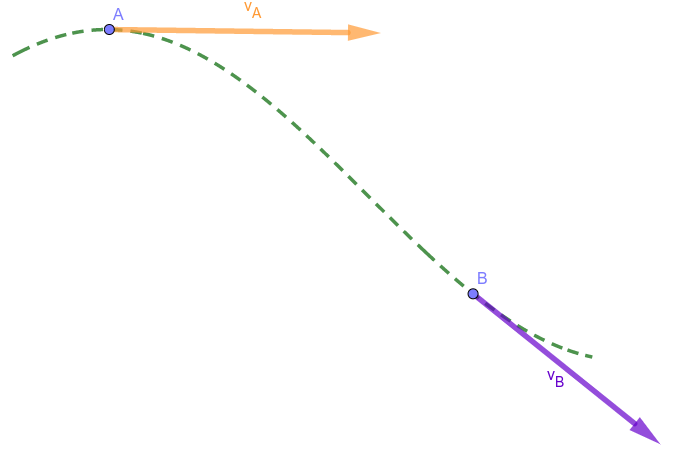
\includegraphics[width=.6\columnwidth]{img/vettorevelocita.png}
\end{figure}


\end{frame}



\begin{frame}
  \frametitle{Modello semplificato}
In questa trattazione daremo un \emph{modello semplificato} del moto di un oggetto che viene lanciato in una certa direzione (una palla, un proiettile, ecc.) e subisce la forza di \alert{attrazione gravitazionale}.\pause\\~\\Ignoreremo l'effetto dell'aria sul corpo, la rotazione del corpo, ecc., perché troppo complessi per le nostre conoscenze attuali.
\end{frame}






\begin{frame}
  \frametitle{Che tipo di moto?}
Un oggetto che viene lanciato con una certa velocità iniziale seguirà una traiettoria diversa a seconda del tipo di lancio (inclinato od orizzontale, da terra o da una certa altezza), ma tutte queste traiettorie hanno in comune il fatto di essere \alert{archi di parabola}.



\begin{columns}
\begin{column}{0.3\textwidth}

\begin{figure}
\begin{tikzpicture}[xscale=.5,yscale=.375]
\node [left] at (0,5) {{\scriptsize $ y $}};
\node [below] at (4.5,0) {{\scriptsize $ x $}};
\draw (0,0) -- (4.5,0);
\draw (0,0) -- (0,5);
\draw[smooth, red, thick, domain=0:4, dashed] plot (\x, {4*\x-\x*\x});
\end{tikzpicture}
\end{figure}

\end{column}
\begin{column}{0.3\textwidth}

\begin{figure}
\begin{tikzpicture}[xscale=.8,yscale=.65]
\node [left] at (0,3) {{\scriptsize $ y $}};
\node [below] at (3,0) {{\scriptsize $ x $}};
\draw (0,0) -- (3,0);
\draw (0,0) -- (0,3);
\draw[smooth, blue, thick, domain=0:2.41, dashed] plot (\x, {1+2*\x-\x*\x});
\end{tikzpicture}
\end{figure}

\end{column}
\begin{column}{0.3\textwidth}

\begin{figure}
\begin{tikzpicture}[xscale=.8,yscale=.4]
\node [left] at (0,5) {{\scriptsize $ y $}};
\node [below] at (3,0) {{\scriptsize $ x $}};
\draw (0,0) -- (3,0);
\draw (0,0) -- (0,5);
\draw[smooth, olive, thick, domain=0:2, dashed] plot (\x, {4-\x*\x});
\end{tikzpicture}
\end{figure}

\end{column}
\end{columns}
\end{frame}





\begin{frame}
\frametitle{Composizione di moti}
Il moto parabolico è ottenuto mediante una \alert<1>{composizione di due moti}:\pause
\begin{itemize}
  \item un moto \alert<2>{rettilineo uniforme} lungo l'asse $ x $;\pause
  \item un moto \alert<3>{uniformemente accelerato} lungo l'asse $ y $ (con accelerazione $ \vec{g} $).\pause
\end{itemize}~\\

Dovremo quindi utilizzare \alert<4>{due velocità diverse per i due moti}: la componente orizzontale $ v_x $ e la componente verticale $ v_y $ del vettore $ \vec{v}_0 $ iniziale.
\begin{center}
\colorbox{blue!30}{$ v_x = v_0 \cos\theta $} ~~~~~~~~ \colorbox{blue!30}{$ v_y = v_0 \sin\theta $}
\end{center}
\end{frame}






\begin{frame}
  \frametitle{Scomposizione del vettore velocità $ \vec{v}_0 $}


\begin{figure}
\begin{tikzpicture}[xscale=1.5,yscale=1.5]
\angolo[black](0,0)(0:63:.5)
\node [left] at (.7,.3) {{\scriptsize $ \theta $}};
\node [left] at (0,3) {{\scriptsize $ y $}};
\node [below] at (5,0) {{\scriptsize $ x $}};
\draw [->] (0,0) -- (5,0);
\draw [->] (0,0) -- (0,3);
\draw[smooth, teal, domain=0:4] plot (\x, {2*\x-.5*\x*\x});
\draw [dashed] (1,2) -- (0,2);
\draw [dashed] (1,2) -- (1,0);
\draw [->,thick,blue](0,0) -- (0,2);
\draw [->,thick,blue](0,0) -- (1,0);
\draw [->,thick,red](0,0) -- (1,2);
\node [below,blue] at (.5,0) {{\scriptsize $ v_x = v \cos\theta $}};
\node [left,blue] at (0,1) {{\scriptsize $ v_y = v \sin\theta $}};
\node [above,red] at (.45,1.1) {{\scriptsize $ \vec{v} $}};
\end{tikzpicture}
\end{figure}



\end{frame}




\begin{frame}
  \frametitle{Equazioni del moto}
  Le equazioni dei moti lungo i due assi sono:
\begin{center}
        \colorbox{blue!30}{$
  \left\{ 
  \begin{array}{l}
  x(t) = v_x t \\
  \quad\\
  y(t) = \dfrac{1}{2}gt^2 + v_y t + y_0
  \end{array}
  \right. 
  $}
    \end{center}
  avendo assunto che il corpo abbia posizione iniziale lungo l'asse $ x $ nulla.\\\pause~\\Sostituendo la prima nella seconda si ottiene un'equazione che fornisce la \alert{traiettoria del corpo}, ed essendo l'equazione di secondo grado la traiettoria sarà \alert{parabolica}.
\end{frame}


\begin{frame}
  \frametitle{Esempio}
  \begin{exampleblock}{Lancio obliquo}
  
\begin{columns}
\begin{column}{0.5\textwidth}

{\small Un sasso viene lanciato da un palazzo alto $ 25 \, m $ con una velocità iniziale di $ 15 \, \frac{m}{s}$ , inclinata di $ 40^\circ $ rispetto all'orizzontale. Dopo quanti secondi e a quale distanza dalla base del palazzo ricadrà il sasso?}

\end{column}
\begin{column}{0.4\textwidth}



\begin{figure}
\begin{tikzpicture}[xscale=.8,yscale=.65]
\node [left] at (0,3) {{\scriptsize $ y $}};
\node [below] at (3,0) {{\scriptsize $ x $}};
\draw [->] (0,0) -- (3,0);
\draw [->] (0,0) -- (0,3);
\draw[smooth, blue, thick, domain=0:2.41] plot (\x, {1+2*\x-\x*\x});
\node [left,blue] at (0,1) {{\scriptsize $ 25 \, m $}};
\node [below,red] at (2.4,0) {{\scriptsize $ ? $}};
\end{tikzpicture}
\end{figure}\pause




\end{column}

\end{columns}

\end{exampleblock}

  

Sappiamo che quando il sasso toccherà terra il valore di $ y $ nel SDR scelto sarà $ 0 \, m $. Poniamo $ y=0 $ nell'equazione verticale del moto e troviamo il valore di $ t $ corrispondente.\pause

Per capire dove ricadrà il sasso, inseriamo il valore di $ t $ appena individuato nell'equazione orizzontale.
\end{frame}




\begin{frame}
  \frametitle{Gittata}
La gittata $ L $ di un lancio è la distanza tra il punto di partenza e il punto in cui il proiettile ricade al suolo.\pause

\begin{figure}
\begin{tikzpicture}[xscale=1.2,yscale=.8]
\node [left] at (0,3) {{\scriptsize $ y $}};
\node [below] at (5,0) {{\scriptsize $ x $}};
\draw [->] (0,0) -- (5,0);
\draw [->] (0,0) -- (0,3);
\draw[smooth, red, thick, domain=0:4] plot (\x, {2*\x-.5*\x*\x});
\draw [|<->|, dashed] (0,-.5) -- (4,-.5);
\node [below] at (2,-.5) {{\scriptsize $ L $ = gittata}};
\end{tikzpicture}
\end{figure}\pause

Se assumiamo che il lancio avvenga da terra (come in figura) e quindi $ y_0 $ si può dimostrare che:
\begin{center}
        \colorbox{blue!30}{$   L = - 2 \frac{v_x v_y}{g} = - 2 \frac{v^2 \sin\theta\cos\theta}{g} $}
    \end{center}




\end{frame}






\begin{frame}
  \frametitle{Dimostrazione}
  Poniamo $ y=0 $ nella seconda equazione per trovare l'istante in cui il corpo si trova al suolo.
\begin{center}
$  \dfrac{1}{2}gt^2 + v_y t = 0 $\\\pause~\\
$ t\left(\dfrac{1}{2}gt + v_y \right) = 0 $\\\pause~\\
$ t =0 $ (inizio del lancio) $ \vee $ $ \dfrac{1}{2}gt + v_y = 0 $ \\\pause~\\
$ t= -\dfrac{2v_y}{g} $
\end{center}\pause
Sostituendo questo valore nella prima equazione otteniamo:
\begin{center}
\colorbox{blue!30}{$   x = - 2 \dfrac{v_x v_y}{g} $}
\end{center}
\end{frame}

\section{Radianti}
\begin{frame}
  \frametitle{Una nuova unità di misura}
  \begin{alertblock}{Attenzione!}
    Gli angoli in fisica sono misurati in radianti, quindi è fondamentale capire questa unità di misura prima di procedere!
  \end{alertblock}
\end{frame}

\begin{frame}
  \frametitle{Definizione di radiante}
\begin{block}{Misura di un angolo in radianti}
    L'ampiezza $ \theta $ di un angolo, espressa in radianti, è data dal rapporto tra l'arco $ l $ e il raggio $ r $ della circonferenza.
        \begin{center}
\colorbox{blue!30}{$ \theta_{rad} = \dfrac{l}{r} $}
\end{center}
  \end{block}
  
\begin{figure}
\begin{tikzpicture}[scale=1.5]
\angolo[blue,thick](0,0)(60:150:1)
\angolo[->,black,thick](0,0)(60:150:.3)
\draw [thick] (0,0) circle [radius=.01];
\draw [thick,purple] (0,0) -- (.5,.866);
\draw [thick,purple] (0,0) -- (-.866,.5);
\node [above,purple] at (.4,.3) {{\scriptsize $ r $}};
\node [above,black] at (-.1,.25) {{\scriptsize $ \theta $}};
\node [above,blue] at (0,1) {{\scriptsize $ l $}};
\draw [thick] (.5,.866) circle [radius=.01];
\draw [thick] (-.866,.5) circle [radius=.01];
\end{tikzpicture}
\end{figure}
\end{frame}

\begin{frame}
  \frametitle{Conversione}
Sappiamo che un angolo di $ 360^\circ $ ha come arco l'intera circonferenza, di lunghezza $ 2\pi r $.{\pause} L'angolo di $ 360^\circ $ in radianti sarà uguale a:
\begin{center}
$ \dfrac{l}{r} = \dfrac{2\pi r}{r} = \dfrac{2\pi \cancel{r}}{\cancel{r}} = 2\pi $
\end{center}\pause
Da qui possiamo dedurre i valori in radianti di altri \emph{archi notevoli}:\\~\\
\colorbox{blue!30}{
\centering\footnotesize 
\begin{tabular}{rccccccccc}
  \textbf{Gradi} & $ 0^\circ $ & $ 30^\circ $ & $ 45^\circ $ & $ 60^\circ $ & $ 90^\circ $ & $ 120^\circ $ & $ 180^\circ $ & $ 270^\circ $ & $ 360^\circ $ \\
  &&&&&&&&&\\
  \textbf{Radianti} & 0 & $ \dfrac{\pi}{6} $ & $ \dfrac{\pi}{4} $ & $ \dfrac{\pi}{3} $ & $ \dfrac{\pi}{2} $ & $ \dfrac{2\pi}{3} $ & $ \pi $ & $ \dfrac{3\pi}{2} $ & $ 2\pi $ \\
\end{tabular}
}
\end{frame}



\section{Circolare}

\begin{frame}
\frametitle{Moto circolare uniforme}
  \begin{block}{Definizione}
    Il moto circolare uniforme è quello di un punto materiale che descrive una traiettoria circolare mantenendo costante il \emph{modulo} del vettore velocità istantanea (cambia invece in ogni istante la \emph{direzione} di tale vettore).
  \end{block}
  
\begin{figure}
\begin{tikzpicture}[scale=1.5]
\draw [] (0,0) circle [radius=1];
\draw [thick] (0,0) circle [radius=.01];
\draw [->,thick,blue] (0,0) -- (.5,.866);
\draw [->,thick,red] ((.5,.866) -- (-.366,1.366);
\node [left] at (0,0) {{\scriptsize $ C $}};
\node [above,red] at (.2,1.1) {{\scriptsize $ \vec{v} $}};
\node [above,blue] at (.1,.3) {{\scriptsize $ \vec{r} $}};
\end{tikzpicture}

$ \vec{r} $ = raggio vettore. $ \vec{r}\perp\vec{v} $
\end{figure}
\end{frame}


\begin{frame}
\frametitle{Periodo e frequenza}
  \begin{block}{Periodo}
    Un moto è periodico quando si ripete uguale dopo un certo intervallo di tempo $ T $, detto \emph{periodo} $ [s] $.
  \end{block}\pause
  \begin{block}{Frequenza}
    La frequenza $ f $ di un moto periodico è il numero di periodi compiuti in $ 1 \, s $ e si misura in $ Hz $ (\emph{hertz}). Vale:
    \begin{center}
\colorbox{blue!30}{$ f = \dfrac{1}{T} $} ~~~ $  [Hz] = \left[ \dfrac{1}{s} \right] = \left[s^{-1}\right] $
\end{center}
  \end{block}

\end{frame}




\begin{frame}
  \frametitle{Modulo del vettore velocità tangenziale}
  Partiamo dalla definizione di velocità:
  \begin{center}
$ v = \dfrac{\Delta s}{\Delta t} $
  \end{center}\pause
  e, considerando che lo spazio percorso in un periodo è un'intera circonferenza:
  \begin{center}
\colorbox{blue!30}{$ v = \dfrac{2\pi r}{T} $}
  \end{center}
\end{frame}

\begin{frame}
  \frametitle{Velocità angolare (1)}
  \begin{block}{Definizione}
    La velocità angolare $ \omega $ di un moto circolare uniforme è il rapporto tra l'angolo spazzato $ \Delta \theta $ e il tempo $ \Delta t $ impiegato dal raggio vettore a spazzare tale angolo.
      \begin{center}
\colorbox{blue!30}{$ \omega = \dfrac{\Delta \theta}{\Delta t}$} ~~~ $  \left[ \dfrac{rad}{s} \right] $
  \end{center}
  \end{block}
  
  
  \begin{figure}
\begin{tikzpicture}[scale=2]
\angolo[->,purple,thick](0,0)(60:150:.5)
\angolo[black,dashed](0,0)(60:150:1)
\draw [thick] (0,0) circle [radius=.01];
\draw [thick] (.5,.866) circle [radius=.01];
\draw [thick] (-.866,.5) circle [radius=.01];
\draw [->,thick,blue] (0,0) -- (.5,.866);
\draw [->,thick,blue] (0,0) -- (-.866,.5);
\node [above,purple] at (-.1,.5) {{\scriptsize $ \Delta \theta $}};
\end{tikzpicture}
\end{figure}
\end{frame}


\begin{frame}
  \frametitle{Esempio}
  \begin{exampleblock}{Calcolo della velocità angolare}
    \small{Un'auto percorre la curva di un incrocio di strade perpendicolari tra loro in $ 4,0 \, s $.
    
    Quanto vale la sua velocità angolare?}
  \end{exampleblock}
\end{frame}


\begin{frame}
  \frametitle{Velocità angolare (2)}
  Considerando che per percorrere un'intera circonferenza ($ \Delta \theta = 2\pi $) è necessario un intero periodo ($ \Delta t = T $), vale:
\begin{center}
\colorbox{blue!30}{$ \omega = \dfrac{2\pi}{T} = 2\pi f $}
\end{center}\pause
Possiamo inoltre esprimere il modulo della velocità tangenziale $ \vec{v} $ in funzione della velocità angolare $ \omega $:
\begin{center}
$ v = \dfrac{2 \pi r }{T} = \left( \dfrac{2\pi}{T} \right)  r = \omega r $
\end{center}
\end{frame}


\begin{frame}
  \frametitle{Esempio}
  \begin{exampleblock}{Calcolo della velocità tangenziale}
    \small{Con riferimento all'esercizio precedente, quanto vale la velocità tangenziale se il raggio della curva è di $ 5,0 \, m $? Esprimi il risultato in m/s e in km/h.}
  \end{exampleblock}\pause

  \begin{center}
    $ v =  0,39 \,\frac{rad}{s} \cdot 5,0 \, m = 1,96 \, \frac{m}{s} = 7,07 \, \frac{km}{h} $
  \end{center} 
\end{frame}




\begin{frame}
  \frametitle{Accelerazione?}
  Sappiamo che:
  \begin{itemize}
    \item un'accelerazione è una \emph<1>{variazione di velocità che avviene in un certo tempo};\pause
    \item \emph<2>{la velocità  è un vettore}, con un'intensità, una direzione e un verso;\pause
    \item nel moto circolare \emph<3>{il vettore velocità cambia in ogni istante}, non in intensità ma in direzione.\pause
  \end{itemize}
  Concludiamo che \alert{nel moto circolare uniforme è presente un'accelerazione}, il cui effetto non è modificare il modulo del vettore $ \vec{v} $, ma la sua \alert{direzione}.
\end{frame}


\begin{frame}
  \frametitle{Accelerazione centripeta (1)}
Tale accelerazione è detta \emph{accelerazione centripeta} (dal latino \emph{centrum}, centro + \emph{petere}, dirigersi) in quanto è sempre rivolta verso il centro della traiettoria\footnote{Vedremo più avanti che questo comporta che la \emph{forza centripeta} non compia lavoro sul corpo, non ne alteri cioè l'energia.} e vale:
\begin{center}
\colorbox{blue!30}{$ a_c = \dfrac{v^2}{r} = \omega^2 r $}
\end{center}
\end{frame}

\begin{frame}
\frametitle{Accelerazione centripeta (2)}

\begin{figure}
\begin{tikzpicture}[scale=2.5]
\draw [dashed] (0,0) -- (.5,.866);
\draw [] (0,0) circle [radius=1];
\draw [thick] (0,0) circle [radius=.01];
\draw [<-,thick,blue] (.125,.2165) -- (.5,.866);
\draw [->,thick,red] ((.5,.866) -- (-.366,1.366);
\node [above,red] at (.2,1.1) {{\scriptsize $ \vec{v} $}};
\node [above,blue] at (.15,.4) {{\scriptsize $ \vec{a}_c $}};
\end{tikzpicture}
\end{figure}
\end{frame}




\begin{frame}
  \frametitle{Forza centripeta}
  Sappiamo dal primo principio della dinamica che se un corpo non è soggetto a forze o la somma delle forze agenti su di esso è nulla, esso rimarrà in quiete o si muoverà di \alert<1>{moto rettilineo} uniforme.\\\pause~\\Per mantenere quindi un corpo in \alert<2>{moto circolare} uniforme è necessaria una forza che agisca verso il centro del moto (causando l'accelerazione centripeta): la \alert<2->{forza centripeta}.\pause
  \begin{center}
\colorbox{blue!30}{$ F_c = ma_c = m\dfrac{v^2}{r} = m\omega^2r $}
\end{center}
\end{frame}


\begin{frame}
  \frametitle{E la forza centrifuga?}
  La forza \emph{centrifuga} non è e in questo momento non può essere oggetto del nostro studio.\\\pause~\\  
  La forza centrifuga è una \emph{forza apparente}, cioè una forza rilevabile solo in un sistema di riferimento non inerziale.\\\pause~\\  
  Esempi di sistemi di riferimento non inerziali sono quelli in cui non vale il primo principio della dinamica: treni che accelerano, automobili che curvano, giostre, ecc.
\end{frame}


\begin{frame}
\frametitle{Esempio}
\begin{exampleblock}{Intensità della forza centripeta}
\small{Un'auto di massa $ 1000 \, kg $ affronta una curva alla velocità di $ 55 \, km/h $. Il coefficiente di attrito tra le gomme e il piano stradale è $ 0,70 $.

Quanto misura il raggio della curva?\hspace*{\fill}[$ 34 \, m $]}
\end{exampleblock}
\end{frame}



\section{Armonico}


\begin{frame}
  \frametitle{Fenomeni}
  Che cosa hanno in comune situazioni come quella di un pendolo, di una massa appesa ad una molla e la corrente elettrica casalinga?
  \begin{columns}
    \begin{column}{0.3\textwidth}
      \begin{figure}
        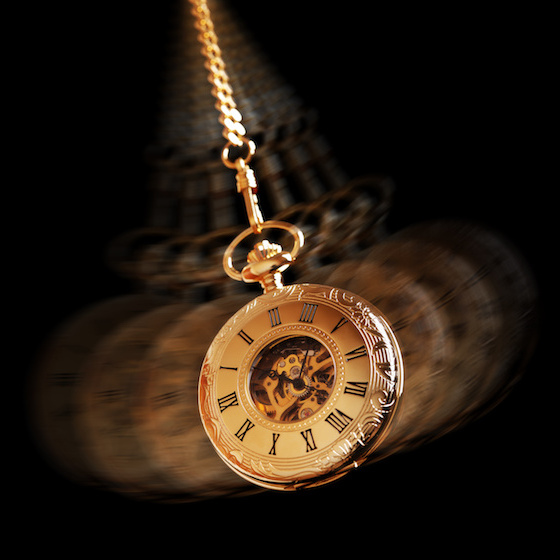
\includegraphics[width=\columnwidth]{img/pendolo.jpg}
      \end{figure}
    \end{column}
    \begin{column}{0.3\textwidth}
      \visible<1->{\begin{figure}
        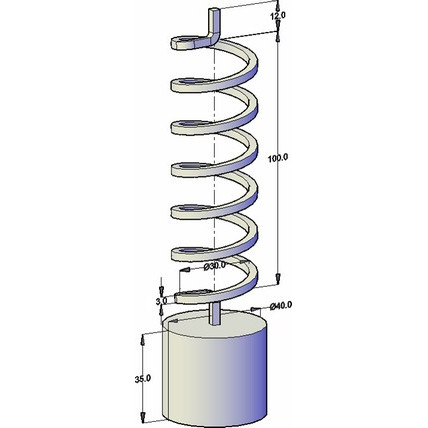
\includegraphics[width=\columnwidth]{img/mollamassa.jpg}
      \end{figure}}
    \end{column}
    \begin{column}{0.3\textwidth}
      \visible<1->{\begin{figure}
        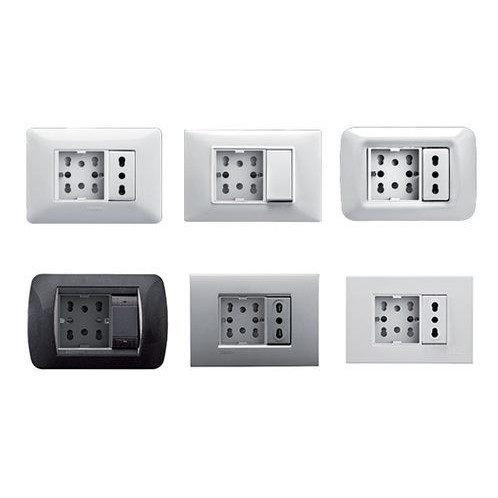
\includegraphics[width=\columnwidth]{img/presa.jpg}
      \end{figure}}
    \end{column}
  \end{columns}\pause
  \begin{center}
  ~
  \end{center}
  Sono tutti esempi di \emph{moto armonico}.
\end{frame}


\begin{frame}
  \frametitle{Il moto armonico}
  \begin{block}{Definizione}
    Il moto armonico è il moto che si ottiene proiettando su un diametro le posizioni di un punto materiale che si muove di moto circolare uniforme.
  \end{block}
\begin{figure}
\begin{tikzpicture}[scale=1.5]
\draw [] (0,0) circle [radius=1];
\draw [thick] (-1,0) -- (1,0);
\draw [dashed] (.5,0) -- (.5,.866);
\draw [dashed] (.866,0) -- (.866,.5);
\draw [dashed] (0,0) -- (0,1);
\draw [dashed] (-.5,0) -- (-.5,.866);
\draw [dashed] (-.866,0) -- (-.866,.5);
\node [below] at (0,0) {{\scriptsize $ Q_4 $}};
\node [below] at (-.866,0) {{\scriptsize $ Q_6 $}};
\node [below] at (-.5,0) {{\scriptsize $ Q_5 $}};
\node [below] at (.866,0) {{\scriptsize $ Q_2 $}};
\node [below] at (.5,0) {{\scriptsize $ Q_3 $}};
\node [above] at (0,1) {{\scriptsize $ P_4 $}};
\node [above left] at (-.866,.5) {{\scriptsize $ P_6 $}};
\node [above left] at (-.5,.866) {{\scriptsize $ P_5 $}};
\node [above right] at (.866,.5) {{\scriptsize $ P_2 $}};
\node [above right] at (.5,.866) {{\scriptsize $ P_3 $}};
\node [right] at (1,0) {{\scriptsize $ Q_1 = P_1 $}};
\node [left] at (-1,0) {{\scriptsize $ Q_7 = P_7 $}};
\angolo[->,purple,thick](0,0)(0:30:1)
\angolo[->,cyan,thick](0,0)(30:60:1)
\angolo[->,red,thick](0,0)(60:90:1)
\angolo[->,teal,thick](0,0)(90:120:1)
\angolo[->,orange,thick](0,0)(120:150:1)
\angolo[->,olive,thick](0,0)(150:180:1)
\draw [->,thick,purple] (1,0) -- (.866,0);
\draw [->,thick,cyan] (.866,0) -- (.5,0);
\draw [->,thick,red] (.5,0) -- (0,0);
\draw [->,thick,teal] (0,0) -- (-.5,0);
\draw [->,thick,orange] (-.5,0) -- (-.866,0);
\draw [->,thick,olive] (-.866,0) -- (-1,0);
\end{tikzpicture}

I punti $ P_n $ sono disegnati a intervalli di tempo uguali.
\end{figure}
\end{frame}


\begin{frame}
  \frametitle{Osservazioni}
\begin{columns}
\begin{column}{0.5\textwidth}


\begin{figure}
\begin{tikzpicture}[scale=1.2]
\draw [] (0,0) circle [radius=1];
\draw [thick] (-1,0) -- (1,0);
\draw [dashed] (.5,0) -- (.5,.866);
\draw [dashed] (.866,0) -- (.866,.5);
\draw [dashed] (0,0) -- (0,1);
\draw [dashed] (-.5,0) -- (-.5,.866);
\draw [dashed] (-.866,0) -- (-.866,.5);
\angolo[->,purple,thick](0,0)(0:30:1)
\angolo[->,cyan,thick](0,0)(30:60:1)
\angolo[->,red,thick](0,0)(60:90:1)
\angolo[->,teal,thick](0,0)(90:120:1)
\angolo[->,orange,thick](0,0)(120:150:1)
\angolo[->,olive,thick](0,0)(150:180:1)
\draw [->,thick,purple] (1,0) -- (.866,0);
\draw [->,thick,cyan] (.866,0) -- (.5,0);
\draw [->,thick,red] (.5,0) -- (0,0);
\draw [->,thick,teal] (0,0) -- (-.5,0);
\draw [->,thick,orange] (-.5,0) -- (-.866,0);
\draw [->,thick,olive] (-.866,0) -- (-1,0);
\end{tikzpicture}
\end{figure}


\begin{figure}
\begin{tikzpicture}[scale=1.2]
\draw [] (0,0) circle [radius=1];
\draw [thick] (-1,0) -- (1,0);
\draw [dashed] (.5,0) -- (.5,-.866);
\draw [dashed] (.866,0) -- (.866,-.5);
\draw [dashed] (0,0) -- (0,-1);
\draw [dashed] (-.5,0) -- (-.5,-.866);
\draw [dashed] (-.866,0) -- (-.866,-.5);
\angolo[<-,purple,thick](0,0)(0:-30:1)
\angolo[<-,cyan,thick](0,0)(-30:-60:1)
\angolo[<-,red,thick](0,0)(-60:-90:1)
\angolo[<-,teal,thick](0,0)(-90:-120:1)
\angolo[<-,orange,thick](0,0)(-120:-150:1)
\angolo[<-,olive,thick](0,0)(-150:-180:1)
\draw [<-,thick,purple] (1,0) -- (.866,0);
\draw [<-,thick,cyan] (.866,0) -- (.5,0);
\draw [<-,thick,red] (.5,0) -- (0,0);
\draw [<-,thick,teal] (0,0) -- (-.5,0);
\draw [<-,thick,orange] (-.5,0) -- (-.866,0);
\draw [<-,thick,olive] (-.866,0) -- (-1,0);
\end{tikzpicture}
\end{figure}
\end{column}
\begin{column}{0.5\textwidth}
Notiamo che la velocità \emph{non è uniforme}: il corpo è più veloce al centro e più lento agli estremi.\\~\\Nei punti di inversione del moto la velocità è nulla.
\end{column}
\end{columns}
\end{frame}




\begin{frame}
\frametitle{Grafico spazio-tempo del moto armonico}
\begin{figure}
  \begin{tikzpicture}[xscale=.4,yscale=1]
\node [above] at (1*pi,1) {{\scriptsize $ T $}};
\node [right] at (2*pi,.5) {{\scriptsize $ A $}};
\node [left] at (0,1.5) {{\scriptsize $ s $}};
\node [below] at (4*pi,0) {{\scriptsize $ t $}};
\draw [->] (-1,0) -- (4*pi,0);
\draw [|<->|, dashed, thick] (0*pi,1) -- (2*pi,1);
\draw [|<->|, dashed, thick] (2*pi,0) -- (2*pi,1);
\draw [->] (0,-1.5) -- (0,1.5);
\draw[smooth, red, thick, domain=0:3.5*pi] plot (\x, {cos(\x r)});
\end{tikzpicture}
\end{figure}
\begin{itemize}
\item $ T $ = periodo $ [s] $ \item $ A $ = ampiezza (raggio della circonferenza) $ [m] $
\end{itemize}
\end{frame}

\begin{frame}
\frametitle{Legge oraria del moto armonico}
\begin{figure}
  \begin{tikzpicture}[xscale=.3,yscale=.75]
\node [above] at (1*pi,1) {{\tiny $ T $}};
\node [right] at (2*pi,.5) {{\tiny $ r $}};
\node [left] at (0,1.5) {{\tiny $ s $}};
\node [below] at (4*pi,0) {{\tiny $ t $}};
\draw [->] (-1,0) -- (4*pi,0);
\draw [|<->|, dashed] (0*pi,1) -- (2*pi,1);
\draw [|<->|, dashed] (2*pi,0) -- (2*pi,1);
\draw [->] (0,-1.5) -- (0,1.5);
\draw[smooth, red, thick, domain=0:3.5*pi] plot (\x, {cos(\x r)});
\end{tikzpicture}
\end{figure}
La curva ha equazione:
\begin{center}
\colorbox{blue!30}{$ s(t) = r \cos (\omega t) = r \cos \left(\frac{2\pi}{T}t\right) $}
\end{center}
$ \omega $ viene anche detta \emph{pulsazione} del moto ed è la velocità angolare del punto che genera il moto armonico.
\end{frame}

\begin{frame}
  \frametitle{Velocità e accelerazione nel moto armonico}
  Velocità e accelerazione sono \alert<1>{diverse in ogni istante} nel moto armonico.{\pause} In particolare:
  \begin{center}
\colorbox{blue!30}{$ v(t) = - r\omega \sin (\omega t) $}
\end{center}\pause
Notiamo che l'accelerazione è sempre diretta in verso opposto rispetto al vettore posizione $ \vec{s} $. Vale:
\begin{center}
\colorbox{blue!30}{$ a(t) = - r\omega^2 \cos (\omega t) $}
\end{center}
\end{frame}





\end{document}
